%DLC development

\begin{frame}{Features of DLC in APP}
    \begin{minipage}[c]{0.64\textwidth}
        \begin{itemize}
            \item Constantly growing precision and data amounts;
            \item Rare events and low statistics;
            \item Call for multi-messenger astrophysics;
            \item Need for various data in analysis;
            \item Data mining in astroparticle data;
            \item Need for advanced storage architectures and smart data selection queries.

        %     \item Experiments improve and are measuring events with greater precision (large amount of data);
        %     \item But not too many events of our interest;
        %     \item[$\Rightarrow$] combined analysis of data from different experiments becomes topical;
        %     \item Astronomical Virtual Observatories (Auger \& IceCube data).


        %     \item  constantly growing precission and data amounts;
        %     \item rare events and low statistics;
        %     \item call for multi-messenger astrophysics;
        %     \item  need for various data in analysis;
        %     \item data mining in astroparticle data;
        %     \item Need for advanced storage architectures and smart data selection queries
        \end{itemize}
    \end{minipage}
    \hfill
    \begin{minipage}[c]{0.35\textwidth}
        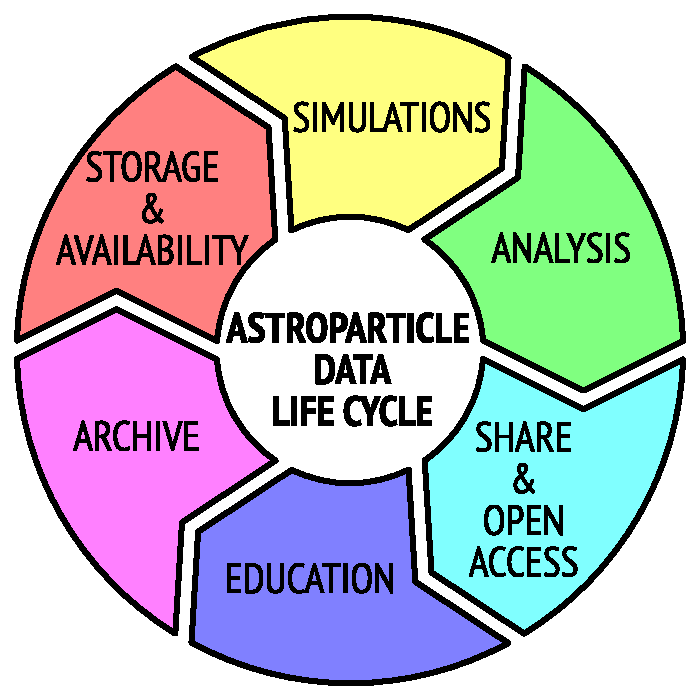
\includegraphics[width=1\textwidth]{pics/ADLC.pdf}
    \end{minipage}
\end{frame}
% 
% \begin{frame}{KASCADE Cosmic-ray Data Center (KCDC) in a nutshell}
%         \tiny
%  \textcolor{red}{the overview is taken from A.Haungs. Rewrite!}
%   \textcolor{red}{Add KCDC logo and scheme!}
%     \begin{itemize}
%              \tiny
%         \item providing open access to astroparticle physics research data
%         as required by funding agencies
%         \begin{itemize}
%             \item data provider
%             \begin{itemize}
%                 \item follows the “Berlin Declaration on Open Data and Open Access”
%                 \item free, unlimited, open access to KASCADE cosmic ray data
%                 \item selection of fully calibrated quantities and detector signals
%                 \item reliable data source
%                 \item guaranteed data quality
%             \end{itemize}
%             \item information platform
%             \begin{itemize}
%                 \item experiment description
%                 \item meta information for data analysis
%                 \item physics background
%                 \item use of modern and open source web technologies
%                 \item tutorials (focused on teachers and pupils)
%             \end{itemize}
%             \item long-term digital data archive
%             \begin{itemize}
%                 \item archive of software and data
%                 \item for the collaboration
%                 \item for the public 
%             \end{itemize}
%         \end{itemize}
%     \end{itemize}
% \end{frame}

\begin{frame}{KASCADE Cosmic-ray Data Center (KCDC)}
    \begin{itemize}
        \small
        \setlength{\itemsep}{0pt}
        \item providing free, unlimited, reliable open access to KASCADE cosmic ray data at \textcolor{blue}{\underline{https://kcdc.ikp.kit.edu}};
        \item almost all KASCADE data is available;
        \item selection of fully calibrated quantities and detector signals;
        \item information platform: physics and experiment backgrounds, tutorials, meta information for data analysis;
        \item archive of KASCADE software and data;
        \item uses modern and open source web technologies.
    \end{itemize}


\includegraphics[height=0.35\textheight]{pics/KCDC-Logo.png}
\hfill
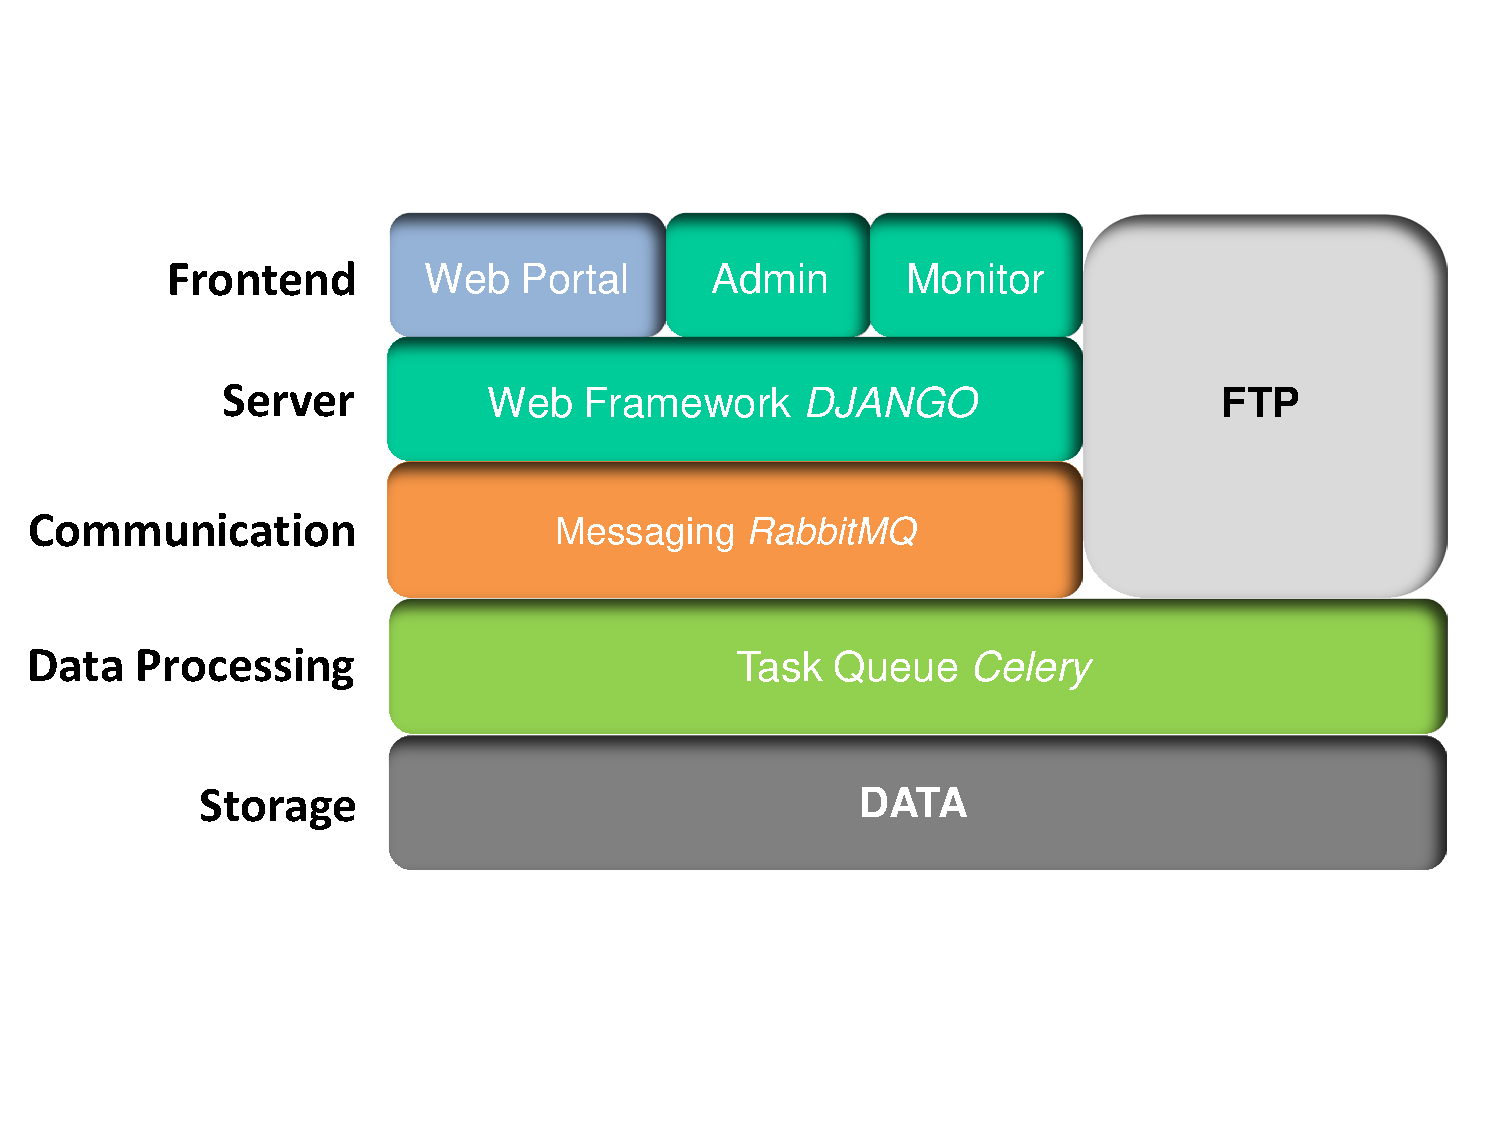
\includegraphics[height=0.35\textheight]{pics/KCDC-IT-Structure.pdf}
\end{frame}


\begin{frame}{DLC Architecture}
\begin{minipage}[c]{0.63\textwidth}
  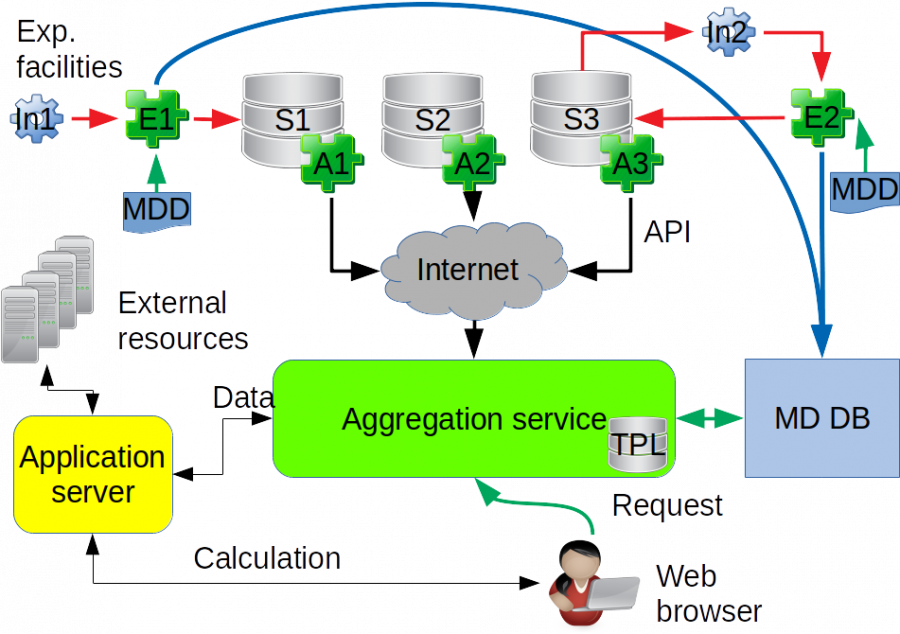
\includegraphics[width=1\textwidth]{pics/arch_appds.png}
\end{minipage}
\hfill
\begin{minipage}[c]{0.36\textwidth}
  \small
  \begin{itemize}
    \setlength{\itemsep}{0pt}
%     \setlength{\parskip}{0pt}
    \item\textbf{Si} — local data storages;
    \item\textbf{Ini} — data sources of different types;
    \item\textbf{MDD} — metadata description;
    \item\textbf{Ei} — metadata extractors;
    \item\textbf{Ai} — adapters, provide API for data access;
    \item\textbf{TPL} — template library;
    \item\textbf{MD DB} — metadata database.
  \end{itemize}
\end{minipage}
\end{frame}
